\documentclass[tikz, border=10pt]{standalone}

\usepackage{tikz}

\begin{document}
    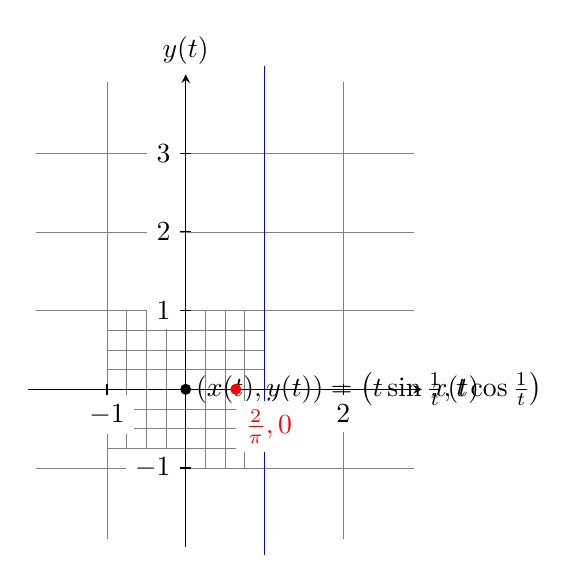
\begin{tikzpicture}
        \draw[style=help lines] (-1.9, -1.9) grid (2.9, 3.9)
            [step=0.25] (-1, -1) grid (1, 1);
        \draw[-stealth] (-2, 0) -- (3, 0) node[right] {$x(t)$};
        \draw[-stealth] (0, -2) -- (0, 4) node[above] {$y(t)$};
        \draw[blue] (1, -2.1) -- (1, 4.1);
        \foreach \pos in {-1, 2}{
            \draw[xshift=\pos cm] (0pt, 2pt) -- (0pt, -2pt) node[below, fill=white] {$\pos$};
        }
        \foreach \pos in {-1, 1, 2, 3}{
            \draw[yshift=\pos cm] (2pt, 0pt) -- (-2pt, 0pt) node[left, fill=white] {$\pos$};
        }
        \fill (0, 0) circle (2pt);
        \draw[thick, parametric, domain=0.4:1.5, samples=200] 
        plot[id=parametric-line] function {(t*t*t)*sin(1/(t*t*t)), (t*t*t)*cos(1/(t*t*t))}
        node[right] {$\left(x(t), y(t)\right) = \left(t\sin\frac{1}{t}, t\cos\frac{1}{t}\right)$};
        \fill[red] (0.63662, 0) circle (2pt) node[below right, fill=white, yshift=-4pt] {$\frac{2}{\pi}, 0$};
    \end{tikzpicture}
\end{document}